\chapter{Funktionen}
\label{chap:methode}

\section{Wie funktioniert die KI?}
Das Verhalten der Technologien werden generell mit Mitteln der Informatik und Mathematik simuliert. Die Maschinen werden für bestimmte Aufgaben trainiert, indem sie mit grossen Datenmengen gefüttert werden und das Muster erkennen. Die KI verwendet künstliche neuronale Netze, um zu funktionieren. Dabei wird die Funktionsweise des Gehirns nachgeahmt. Der Unterschied, das Gehirn kann viel mehr leisten als alle Computer. "Computer stellen diese Informationsverarbeitung  des Gehirns durch künstliche neuronale Netze nach. Informationen werden als Input auf der einen Seite eingegeben, verarbeitet und das Ergebnis wird auf der anderen Seite als Output wieder ausgegeben. Solche Systeme setzen sich aus sogenannten Algorithmen zusammen"\citep{ai-genius-community}.

\begin{figure}[h]
    \centering
    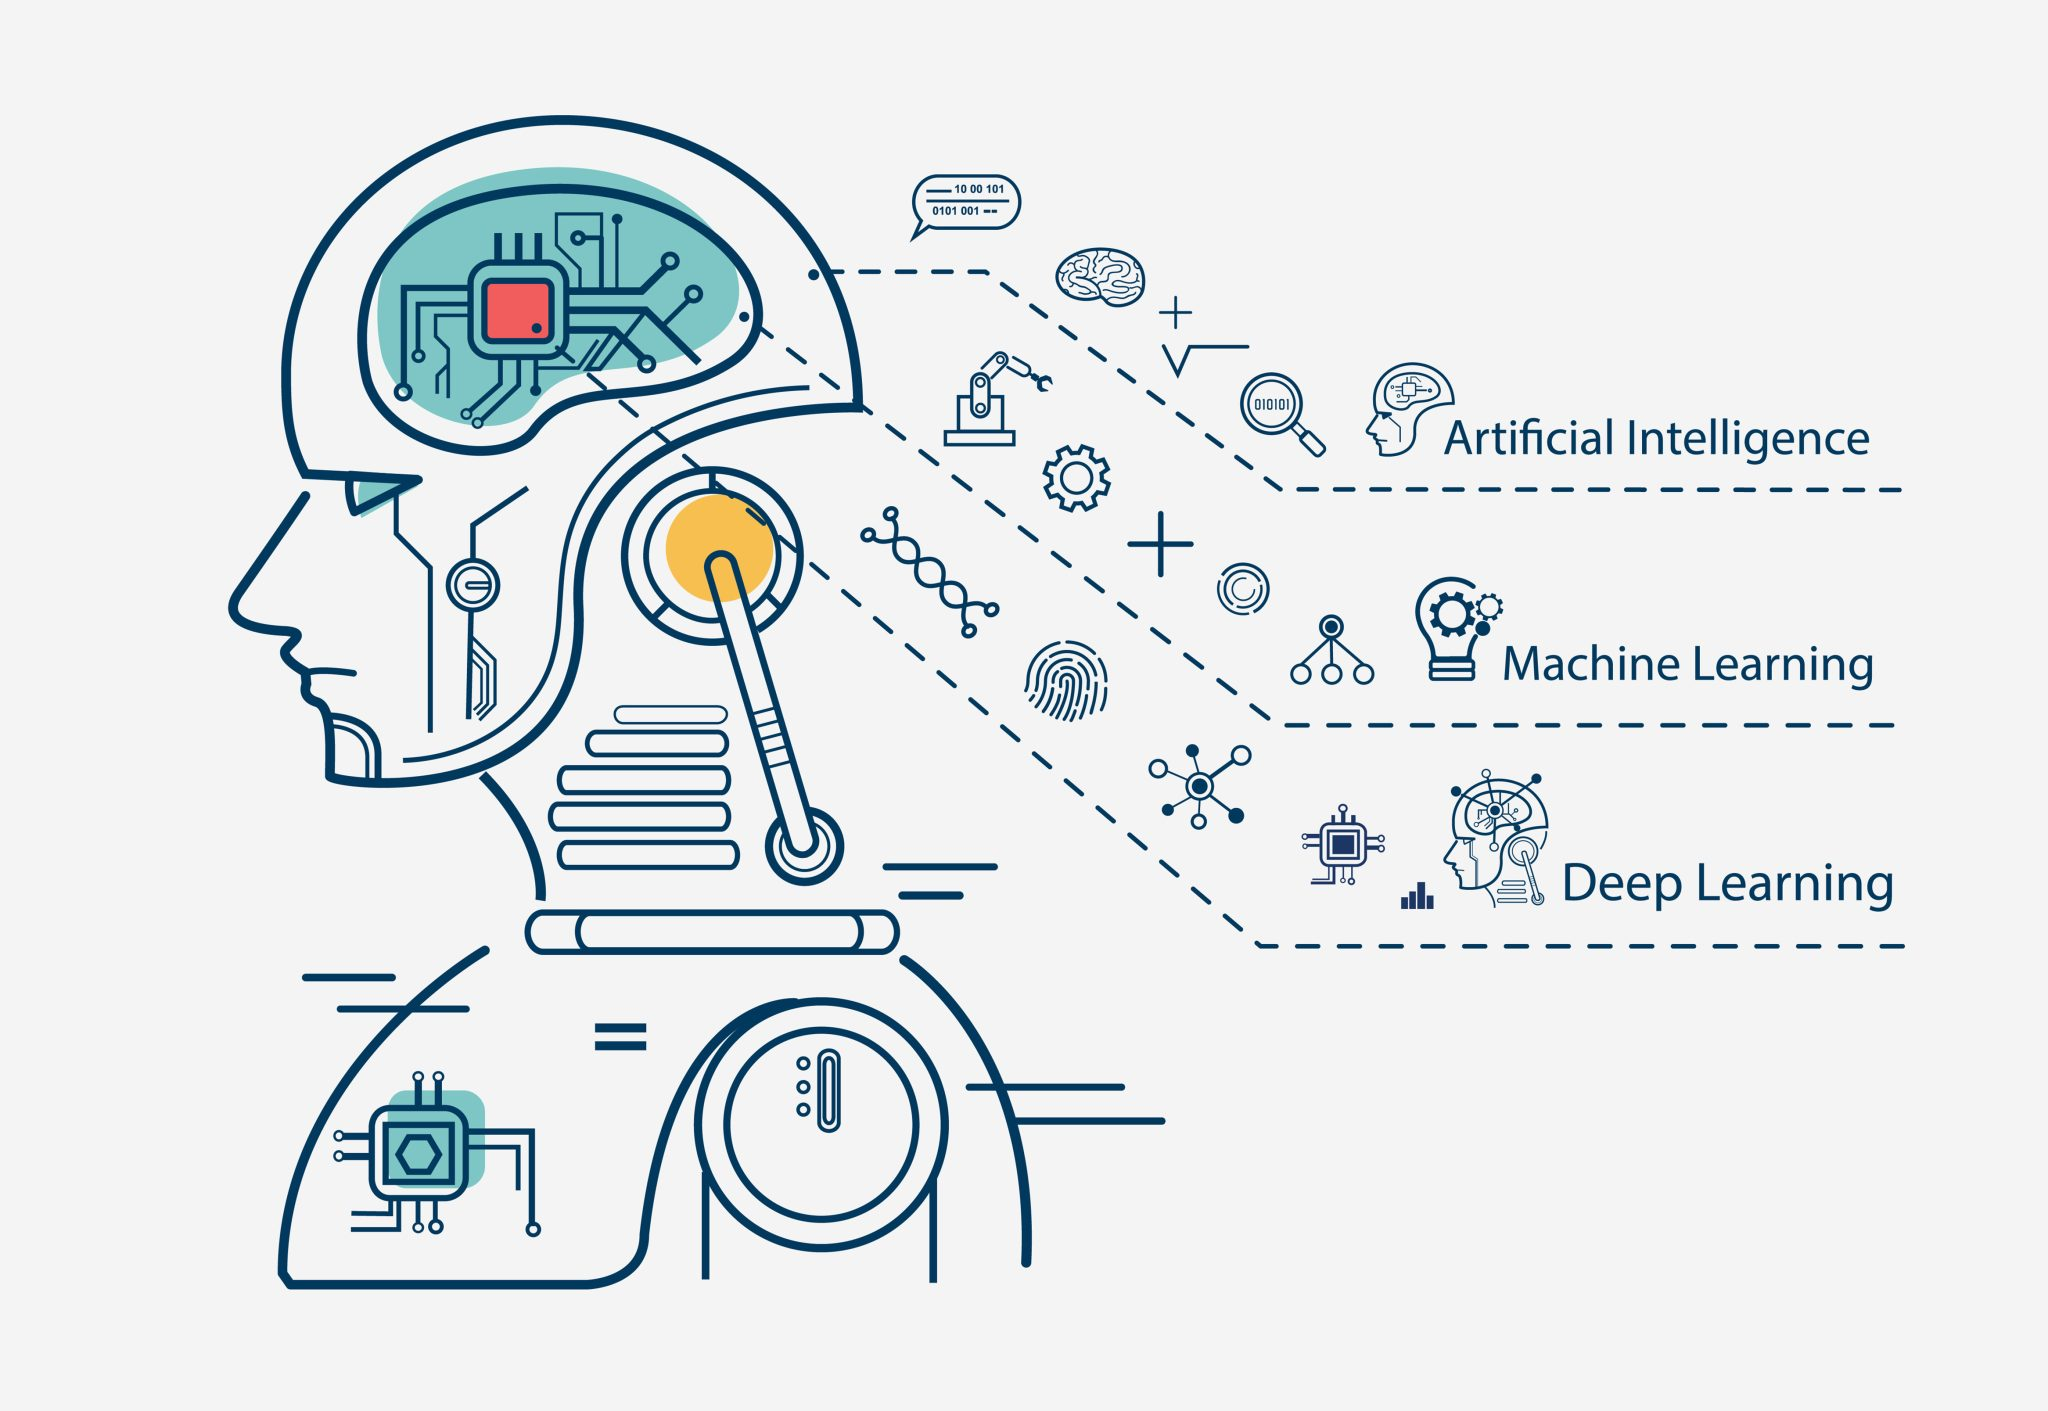
\includegraphics[width=0.5\textwidth]{AI.jpeg} 
    \caption{Bereiche der KI}
    \label{fig:ai}
\end{figure}

\section{Algorithmus}
Ein Algorithmus kann als Anleitung betrachtet werden, das einem Computer sagt, was er machen muss, um eine Aufgabe oder Problem zu lösen. Also muss der Computer wissen, was wir von ihm wollen, bevor er die Aufgabe erledigen kann. Dies wird von IT-Spezialisten programmiert, die dem Computer erklären, was sie von ihm erwünschen und Anweisungen geben, was das System machen soll.

\section{Deep Learning}
"Deep Learning" (deutsch: mehrschichtiges Lernen oder tiefgehendes Lernen)ist eine Kategorie des maschinellen Lernens.
Im Prozess "Deep Learning"   wird dem Computer beigebracht, wie man komplexe Muster aus grossen Datenmengen verstehen kann, indem Schichten von künstlichen neuronalen Netzwerken verwendet werden. Die Konfiguration der Neuronen im Netzwerk basiert auf das Training mit grossen Datenmengen.

\section{Machine Learning}
Ein weiterer wichtiger Begriff im Bereich der Künstlicher Intelligenz ist das "Machine Learning" (deutsch: Maschinelles Lernen), die Begabung des Computers aus Erfahrungen zu lernen und Erkenntnisse aus Daten zu gewinnen, ohne dafür extra programmiert zu sein.